\section{Simulation Setup}

In order to assess the performance of the different fleet sizes and control
algorithms a novel scenario for the city of Zurich, Switzerland is set up
for the MATSim transport simulation framework and a theoretical fleet sizing
according to \citep{spieser2014toward} is performed.

% Commented to reduce works /sh
%The section is structured as follows:
%First, we give an overview about the used simulation components, second, we specify
%the scenario and finally, we provide fleet sizing results from the theoretical
%methodology presented in \citep{spieser2014toward}.

\subsection{MATSim and AMoD Simulation}

MATSim \citep{Horni2015} is an agent-based transport simulation framework that makes it possible
to simulate large numbers of agents representing a real population in a traffic environment. Similar to reality, each agent has a daily plan with activities
that he wants to perform for a certain duration and finish at a specific time of
the day. Since these activities take place at different locations in the scenario,
agents need to move from activity to activity. By default, MATSim allows the
simulation of car traffic, public transit and slow modes such as going by bike
or walking. Network-based modes, such as private cars are simulated in a time-step
based manner in a network of queues with all participants at the same time. This
way it is possible that congestion emerges and  that agents may arrive late at their
activity locations. While MATSim provides more functionality, e.g. the replanning
of agents plans to adapt to the traffic conditions that they perceive, only the
network simulation is used in this research.

An extension developed in \cite{horl_abmtrans17} is used to add automated taxis to the set
of available travel modes. A virtual dispatcher, for which
different algorithms are used in this study, controls a fleet of AVs.
Whenever an agent wants to depart from his current activity location by
AV, a request is issued to the dispatcher and saved.  The choice which vehicle to send and when is completely defined
by the dispatching algorithm. Once the vehicle arrives at the customer's location
he is picked up, the AV drives to the destination and finally drops him off. Then,
the vehicle is available for dispatching again. Alternatively, vehicles can be
rebalanced, which simply means that the dispatcher gives an AV the instruction
to drive to a different location. All of this is performed in the MATSim traffic
simulation such that AVs suffer from congestion as any other vehicle.

% Commented out to save words
%It should be noted that AVs drive directly to the locations where agents finish and
%start their activities. So far no mechanism is implemented that would allow them
%to meet at optimized locations (e.g. a high-capacity avenue instead of a small
%alley).

\subsection{Scenario Definition}

For Switzerland the Microcensus on mobility and transport \cite{microcensus} is
available, which features the daily travel patterns of 60,000 Swiss residents.
It is the basis for a readily available agent population of
Switzerland, which reproduces the demographic attributes and travel patterns
in the country to great detail \cite{ivtbaseline}.

\begin{figure}[h]
\begin{center}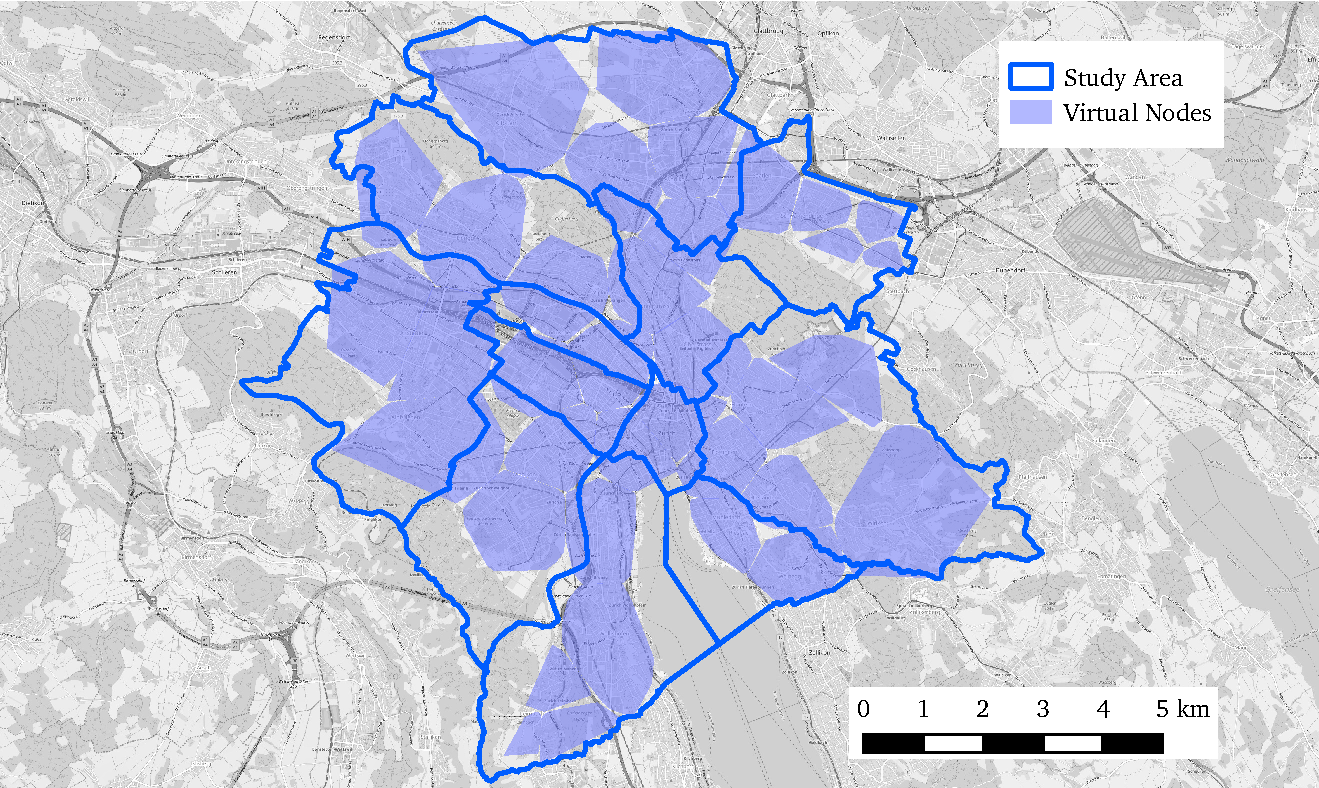
\includegraphics[width=1.0\textwidth]{figures/map.pdf}\end{center}
\caption{The study area covering the 12 districts of Zurich and the nodes of the
virtual network for the rebalancing algorithms.}
\label{fig:study_area_vnodes}
\end{figure}

Additional modifications are applied to this population of around 8 million
agents to make it suitable for the study at hand. First, a best-response routing
of the travels of all agents is performed to find all agents that interfere
with the study area, which has been defined to be the 12 districts of Zurich (Figure \ref{fig:study_area_vnodes}).
All agents which do not interact with that region (i.e. do not perform an activity within
the area and do not cross the area) are deleted from the population as they do
not contribute congestion in the area. Finally, a 1\%
sample of the remaining agents is created. The rather extensive downscaling becomes necessary for the computationally
demanding algorithms, given that they need to be performed hundreds of times faster
than reality to allow for multiple runs and iterations.

%In order to define the travel demand for the fleet of automated vehicles, agents
%are tagged as whether they are viable for using an automated vehicle or not. Pedestrians
%and cyclists are not simulated at all in this work since they do not contribute to congestion in the current version of the framework.

An agent that travels at least once by private car during the simulation is tagged
as an AV user \textit{only} if all of the legs in the agent's plan take place
within the study area. This constraint makes sure that no unrealistic travel
plans are generated, where an agent performs his first leg by AV although his
private car is at home and then wants to depart at the next location with that
car. Finally, the ``car'' legs of all viable agents are converted to the ``av'' mode.
All other legs are kept as before, i.e. short legs that are assigned the ``walk''
mode initially are still performed in this mode.

For agents that use public transit, the procedure is different. Here, any leg
that is performed by the ``pt'' mode in the original population is converted to ``av''
if it lies within the study area. As for car users, connecting non-motorized
legs are kept fixed.

This way a demand for Zurich is generated where each leg that possibly
\textit{can} be performed using an AV \textit{is} performed by AV. In that sense we
simulate a scenario where 100\% of the AV travel demand must be served by the
dispatchers.

To summarize, the 8,230,971 agents in the population are decimated to
1,935,400 agents, which interfere with the study area. From this set of agents
a 1\% sample has is drawn, leading to 13,141 agents that mainly constitute
background traffic for congestion. Among those are 970 agents that are viable for the AV
service. The plans of these agents contain 2,096 trips that are to be served by
AVs. In reality, this scaled service would hence need to serve 209,000 requests by
97,000 persons.

\subsection{Theoretical Fleet Sizing}

% Commented out to save words. I thin kwe explain this further up already. /sh
%Both the capital cost of an AMoD system and the service rates are highly dependent
%on the fleet size which makes fleet sizing an important aspect of AMoD system design.
%If the fleet size is chosen too small, then the service levels will be unacceptable. If the fleet size is chosen too large, the cost of the system becomes unbearable due to low utilization rates.

Fleet sizes can be estimated using simulations, as for instance done in
\citep{bischoff2016simulation}. Despite the accuracy of these
simulation results, they do not provide insights into the fundamental
properties influencing the relationship between fleet size and performance metrics.

For this reason we implement theoretical results from \citep{spieser2014toward}
for the case of Zurich. The authors present two methods for fleet size evaluation.
The first method estimates the theoretical minimum fleet size to stabilize
the system, i.e. ensure that the number of open requests stays bounded at
all times. To do so, for every vertex $i$ and timestep $\delta_t$ the added
unserved mileage per timestep is calculated as
$\lambda_i \cdot ( \bar{d}_{OD,i}  + \bar{d}_{EMD,i})$ where $\bar{d}_{OD,i}$
is the average distance per trip and  $\bar{d}_{EMD,i}$ the earth mover's
distance per vehicle in the timeslice. $\bar{d}_{OD,i}  + \bar{d}_{EMD,i}$
represents the average distance that has to be driven per request. A total of
$m$ vehicles at an average speed of $v$ are collectively able to reduce this
 added mileage at a rate of $m \cdot v$, this quantity has to be larger than the
 added unserved mileage per timestep. For the scenario of this work the
 minimum fleet size compute with this measure are $4271$ vehicles, which
 can be seen as a non-tight lower bound. [TODO: The plots in report.html say
 2800? /sh]

While the knowledge of the minimum fleet size is useful, it does not reveal
the relation between service level and fleet size, especially to what number
the fleet size has to be augmented before further addition of vehicles will
not result in a significant decreaes in wait time. In \citep{zhang2016control}
 a method is presented of how an AMoD system can be cast in a Jackson network.
 For such networks, queuing theoretical results allow for the computation of
 performance measures such as vehicle wait times, queue lengths or
 availabilities at vertices. The quantity of interets is the availability
 of a vehicle at a vertex, which is the probability that at least one idle
 vehicles is at that vertex. Computation of the mean availability of all
 timesteps and vertices as a function of the fleet size for Zurich results
 in the curve shown in \ref{fig:performanceavailability}. Note that these results
 are purely theoretical and can be derived solely from input data without performing simulations.
 Therefore they can serve as a measure of accuracy for the simulation results.

For the peak case, the increase of the number of vehicles up to a fleet size of $15,000$ results
in a availability rising from $0$ to $~0.85$. The addition of another $15'000$ vehicles does only
increase the availability by $~0.05$ to $~0.90$. This corresponds well to the wait times observed
 in simulation shown in figure \ref{fig:mean_peak_waiting_times}. The simulated wait times
 decrease significantly up to a fleet size of $15,000$ before saturating.
 [TODO: Reformulate this? Looking at the wait time plot I don't really see saturation... /sh]
